
% ----------------------------------------------------------------------
\introduction
\label{sec:intro}
% ----------------------------------------------------------------------

At the Last Glacial Maximum (LGM), glaciers of a size comparable to the present Greenland and Antarctic ice sheets covered parts of Northern America (Laurentide, Cordilleran and Innuitian ice sheets) and Northern Eurasia (Fennoscandian Ice Sheet). Numerical modelling of these former ice masses allows for a comparison between glaciological theories embedded in the models and geomorphological traces underpinning palaeo-glaciological reconstructions. Yet, a major obstacle in this exercise resides in large uncertainties concerning climate forcing, typically temperature and precipitation data, needed by numerical glacier models \citep{hebeler-etal-2008}. This includes uncertainty in representation of Earth's present climate in regions of poor station coverage, and even larger uncertainty concerning accurate reconstructions of past climate change.

Arguably the most physically sound way to force an ice sheet model in the past is to couple it with a General Circulation Model (GCM) \citep{yoshimori-etal-2001,calov-etal-2002,abeouchi-etal-2007,charbit-etal-2013}. However the computational demand of GCMs is such that only models of intermediate complexity can run on the time-scales of tens of thousands of years characteristic of ice sheet growth and decay.

%Irina  I think it would be reasonable to discuss the limitations of GCM in this context

Climatologies obtained from uncoupled GCM palaeo-climate simulations such as produced within the PMIP project \citep{joussaume-taylor-1995} provide a more accurate representation of past climate and are commonly used to force ice sheet models. Because they are only available for specific periods of time, they require either an assumption of steady-state \citep{huybrechts-tsiobbel-1996}, or interpolation through time between climatologies from different periods, which can be linear \citep{charbit-etal-2002}, or modulated by a ``glacial index'' weighting function derived from ice core $\delta^{18}$\,O records \citep{marshall-clarke-1999,tarasov-peltier-2004,zweck-huybrechts-2005,gregoire-etal-2012}. An important drawback in this approach is that palaeo-climate simulations themselves rely on global ice sheet reconstructions such as the ICE-4G \citep{peltier-1994} for their surface topographic boundary condition. This indirectly controls subsequently modelled ice sheet geometries, whose spatial extent tend to conform to these reconstructions.
\julien[noline]{Should this literature list be extended to studies not covering North America?}

The other side of the coin is that avoiding this circular dependence unfortunately goes hand-in-hand with a need for simplifying assumptions on Earth's past climate. They include energy balance modelling approaches \citep{tarasov-peltier-1997} and geographic parametrizations of surface mass balance \citep{robert-1991} or climate forcing \citep{johnson-fastook-2002}. Standing on a middle ground, temperature offset methods \citep{greve-etal-1999,bintanja-etal-2005} make use of the high level of detail available in present climate datasets such as gridded observation datasets, GCM output or reanalyses, while using simplifying representations of past climate deviations from this present state.

Here, we propose to address some of the uncertainties concerning climate forcing of numerical glacier models by evaluating their response, in terms of glacier extent, to inputs from several climate datasets. Few studies of this kind are presently available. \citet{quiquet-etal-2012} assessed the sensitivity of a Greenland ice sheet model to various atmospheric forcing, including a regional parametrization \citep{fausto-etal-2009}, output from several GCMs and a climate reanalysis. \citet{rodgers-etal-2004,charbit-etal-2007} tested the sensitivity of a model of the Northern Hemisphere ice sheets to different PMIP LGM simulations. Here, to limit degrees of freedom in our model, and obtain results independent from palaeo-ice sheet reconstructions such as the ICE-4G, we use a simple temperature offset approach similar to \citep{greve-etal-1999,bintanja-etal-2005} and assess ice sheet model sensitivity to the choice of present-day climate data. Rather than using GCM output, we force our model with climate reanalysis data, which include observational information through data assimilation \citep{bengtsson-etal-2007}. Furthermore, we focus our study regionally to the former Cordilleran Ice Sheet in Northern America.

\begin{figure}[t]
	\vspace*{2mm}
	\begin{center}
		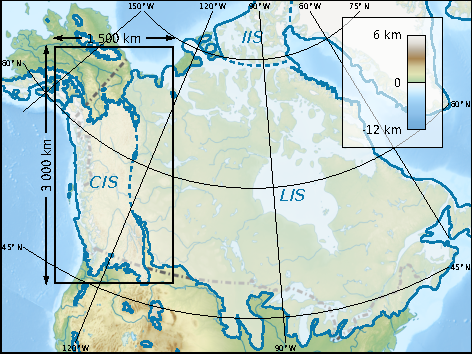
\includegraphics[width=8cm]{cordillera-climate-locmap}
	\end{center}
	\caption{Shaded relief map of northern North America. The frame delimits this study's modelling domain. The outlines of the former ice sheets depict ice cover at 14\,$^{14}$C\,ka\,BP (16.8\,cal\,ka\,BP) after \citet{dyke-2004}. The background map was made with ETOPO1 \citep{data:etopo1} and Natural Earth Data \citep{data:naturalearth}.}
	\label{fig:locmap}
\end{figure}

The Cordilleran Ice Sheet (Fig.~\ref{fig:locmap}) covered an area that presently experiences strong regional variations in climate. In a numerical modelling perspective, it is one of the least studied palaeo-ice sheets of the Northern Hemisphere, despite the fact that significant geomorphological data is available to constrain its extent \citep{jackson-clague-1991,dukrodkin-1999,kaufman-manley-2004,kleman-etal-2010,margold-etal-2011}. Although the Cordilleran Ice Sheet was not the primary target of these simulations, it has previously been modelled as part of efforts to model ice sheets in North America \citep{marshall-clarke-1999,calov-etal-2002,tarasov-peltier-1997,tarasov-peltier-2004,gregoire-etal-2012}, the Northern Hemisphere \citep{huybrechts-tsiobbel-1996,greve-etal-1999,charbit-etal-2002,charbit-etal-2007,charbit-etal-2013,johnson-fastook-2002,rodgers-etal-2004,bintanja-etal-2005,zweck-huybrechts-2005,abeouchi-etal-2007} or world-wide \citep{yoshimori-etal-2001}. While these studies reproduce the magnitude of North American glaciation at the Last Glacial Maximum (LGM) reasonably well, there exist a tendency in simulations independent from ice sheet reconstructions such as the ICE-4G to predict excessive ice cover in parts of northern Yukon Territory and continental Alaska that have remained ice-free throughout the Pleistocene \citep{dukrodkin-1999,kaufman-manley-2004}.

Here we use a Parallel Ice Sheet Model \citep[PISM,][]{web:pism} \julien{Recommended by \url{http://www.pism-docs.org/wiki/doku.php?id=citing_pism}} to simulate the extent and thickness of Cordilleran Ice Sheet at the LGM. We force our model with multiple climate datasets and compare our results to the mapped LGM ice sheet margin from \citet{dyke-2004}. To our knowledge, this is the first modelling study which specifically focus on the Cordilleran Ice Sheet since the one by \citet{robert-1991}. While \citet{robert-1991} modelling domain covered only the southern part of the ice sheet, our model also includes higher resolution and an improved treatment of ice thermodynamics and bedrock response due to large advances made in ice sheet modelling since then. Model set-up is presented in section~\ref{sec:model} and climate forcing in section~\ref{sec:climate}. Results are exposed in section~\ref{sec:results} and discussed in section~\ref{sec:discussion}.
